\documentclass[12px,oz]{report}

\usepackage [english]{babel}
\usepackage [autostyle, english = american]{csquotes}
\MakeOuterQuote{"} % allow usage of "x" instead of ``x''

\usepackage{placeins}
\usepackage{xr-hyper} % must be before hyperref
\usepackage[hidelinks]{hyperref}
\usepackage{graphicx}
\usepackage{pdflscape}
%\usepackage{oz} % conflicts with siunitx
\usepackage{float}
\usepackage{titlesec}
\titleformat{\chapter}[hang] % remove "Chapter N" before chapter name
{\Huge\bfseries}{\thechapter.\hspace{20pt}}{0pt}{\Huge\bfseries}
\titlespacing*{\chapter}{0pt}{10pt}{5pt}


\usepackage[margin=1in]{geometry} % margin!
\usepackage{listings}
\usepackage[dvipsnames]{xcolor}

% for SI units
\usepackage[binary-units=true, detect-all]{siunitx}	

\usepackage{amsmath} % \text{}

\usepackage{longtable}

\usepackage[skip=4pt]{caption} % make captions closer to picture

\usepackage{setspace}
%\singlespacing
\onehalfspacing

\setcounter{secnumdepth}{3} % set subsubsections to be numbered as well

% when using the english language, autoref to subsection and section simply writes "section" instead of using the prefix
\addto\extrasenglish{
	\let\subsectionautorefname\sectionautorefname
	\let\subsubsectionautorefname\sectionautorefname
}

% Header and footer
\usepackage{lastpage}
\usepackage{fancyhdr}
\cfoot{\thepage\ of \pageref{LastPage}}

% Subfigure
\usepackage{caption}
\usepackage{subcaption}

% remove new page after chapter
\usepackage{etoolbox}
\makeatletter
\patchcmd{\chapter}{\if@openright\cleardoublepage\else\clearpage\fi}{}{}{}
\makeatother

% custom functions
\newenvironment{enumerateSmall}%
{\vspace{-5mm}
	\begin{enumerate}%
		\setlength{\itemsep}{0pt}%
		\setlength{\parskip}{0pt}}%
	{\end{enumerate}}

\newenvironment{itemizeSmall}%
{\vspace{-5mm}
	\begin{itemize}%
		\setlength{\itemsep}{0pt}%
		\setlength{\parskip}{0pt}}%
	{\end{itemize}}

\begin{document}	
\pagenumbering{roman} % "gobble" can be used if no pagenumbering is needed	
% TITLE PAGE
	\begin{titlepage}
		\centering
		\vspace*{3\baselineskip}
		{\Huge \bfseries Parallel Programming}
		\rule{\linewidth}{0.5mm}
		%\vspace*{1\baselineskip}\\
		\LARGE
		Reading Course
		\\
		\null\vfill
		\begin{flushleft} \large
			au503241 \hspace*{2em} \  Frederik Andersen\\
			au500070 \hspace*{2em} \  Mathias Jessen\\
			au501580 \hspace*{2em} \  Michael Ilkiv Misbih\\
			au501465 \hspace*{2em} \  Morten Morberg Madsen\\
			au505313 \hspace*{2em} \  Thomas Holm Nielsen\\
			\vspace{100pt}
			Supervisor:\hspace{94pt}  Date: \\
			Kim Bjerge \hspace{90pt}  \today\\
		\end{flushleft}
		\vspace*{6\baselineskip}
	\end{titlepage}

\tableofcontents
\clearpage
\pagenumbering{arabic}
\cleardoublepage

\chapter{Programming Model}
\label{ch:programming-model}
The \cuda{} programming model, is a heterogeneous model where both the CPU and the GPU are used.
In this context \textit{host} refers to the CPU and \textit{device} refers to the GPU and their respective memory.
The code run on the host also manages memory on the device and launches \textit{kernels} to be executed on the device.
The host and device are physically separated, which means that the host execution can run in parallel with the kernel execution on the device.
Kernels can briefly be described as functionality being executed by multiple threads in parallel on the device.

\noindent A typical sequence of operations performed in the \cuda{} programming model is as follows:
\begin{enumerateSmall}
	\item Allocate and initialize host and device memory
	\item Transfer data from host to device
	\item Execute kernel(s) on the device
	\item Transfer result(s) from device to host
\end{enumerateSmall}
The operations involved is described in details in the following sections.
The \cuda{} examples are written in "\cuda{} C", which is an extension to ANSI C, but the principles are generic and can be applied in all \cuda{} programming languages.



\chapter{Parallel Communication Patterns}
\label{ch-patterns}
In parallel computing tasks (threads) need to work together to solve a given problem. 
To be able to solve a problem the different tasks need to communicate with each other.
There are different parallel communications patterns such as map, transpose, gather and stencil.
Such communication patterns are essential for implementing more complex parallel algorithms.
	
	\section{Map}
	\label{sec-map}
	In the map communication pattern each tasks reads and writes to specific data elements in memory.
In its simplicity, the same function or computation is done on each piece of data as seen in bla. bla.

---add fig here

In the this way there is a one-to-one correspondence between the input and output.

This corresponds to that one thread will be doing each task in CUDA.
An example is seen listing bla. bla.

---add code

Here the kernel is launched in one block which spawns 64 threads and each thread does the same computation which is to square its thread id.
	
	\section{Gather}
	\label{sec-gather}
	The gather communication pattern gathers input data elements together from different places in memory and computes a single output result.
This is different from the map pattern since this pattern maps multiple inputs to a single output.
In this way the gather pattern has a many-to-one correspondence between inputs and outputs as can be seen in \autoref{fig:gather}.

\begin{figure}[ht]
	\centering
	\fbox{
		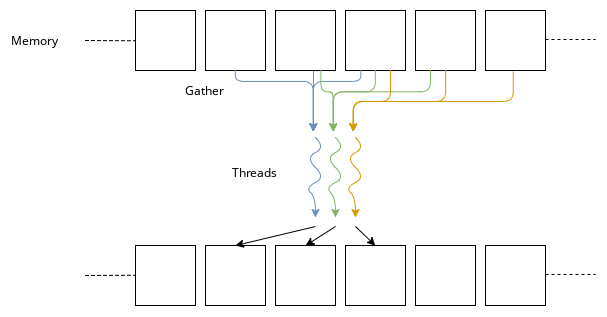
\includegraphics[width=0.75\textwidth]{figs/parallelgather.png}
	}
	\caption{Gather Pattern}
	\label{fig:gather}
\end{figure}

This parallel communication pattern can for instance be applied to image processing applications such as implementing blurring, sharpening, edge detection and more on an image.
This is done by 'sliding' a \textit{kernel} \footnote{Sometimes also called a \textit{convolutional matrix} or \textit{mask}} over the entire image to get a new image with a desired effect.
The effect which is applied to the new image is determined by the values in the kernel, but the parallel pattern which is used to implement this is the same, namely the gather pattern.
An example of applying a kernel to an image is seen in \autoref{fig:kernel}.
\begin{figure}[ht]
	\centering
	\fbox{
		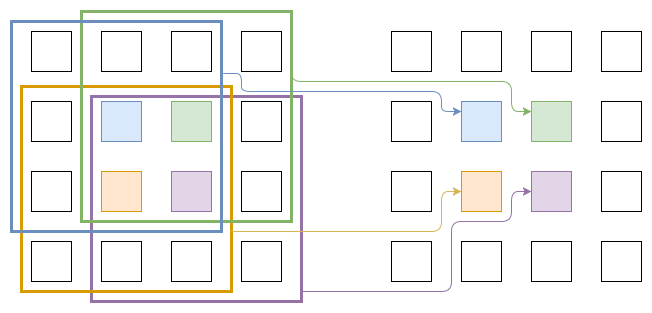
\includegraphics[width=0.6\textwidth]{figs/parallelblur2.png}
	}
	\caption{Example of a kernel operation}
	\label{fig:kernel}
\end{figure}
Using such a parallel communication pattern can vastly improve the computation time of applying for instance a kernel to an image.
Say that with a kernel with $\mathtt{NxN}$ dimensions and an image with $\mathtt{K}$ pixels the running time would be $\mathtt{O(N\cdot K)}$ on serial processor compared to $\mathtt{O(N)}$ in parallel, assuming that $K$ threads can be spawned on the GPU.

%TODO: make small code example of gather
	
	\section{Scatter}
	\label{sec-scatter}
	The scatter communication pattern reorganizes data and writes a single input data element to a single or multiple different output element(s) in memory.
This communication is used when a parallel tasks needs to write its result to a specific or multiple output elements.
It is similar to gather but instead it has a one-to-one/one-to-many correspondence between input and output(s) as seen in \autoref{fig:scatter}.
\begin{figure}[ht]
	\centering
	\fbox{
		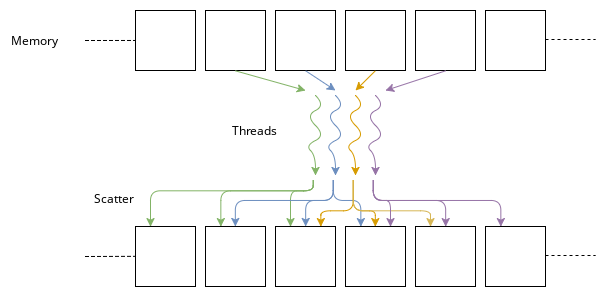
\includegraphics[width=0.6\textwidth]{figs/patterns/parallelscatter.png}
	}
	\caption{Scatter Pattern}
	\label{fig:scatter}
\end{figure}
\autoref{fig:scatter} suggests that there might be a synchronization issue which could lead to a \textit{data race}.
The problem is that several threads will very likely try to write to the same place in memory.
Say for instance that each thread has to increment a variable in memory which can be accessed by any thread.
This increment might not be correct because the variable might have been updated by another thread \textit{after} the variable has been read, which leads to data inconsistency.
This can be avoided by synchronizing threads or declaring the memory section as atomic.

The scatter pattern can for instance be used in combination with the gather pattern for representing sparse matrices which is more thoroughly described in section ?? bla. bla.

	
	\section{Stencil}
	\label{sec-stencil}
	The stencil communication pattern is a special case of the gather pattern.
The stencil pattern reads multiple elements in memory defined by some specific offset or pattern to a given input.
This offset or pattern defines specific characteristics of a stencil.
Examples of specific stencils are \textbf{2D/3D von Neumann} and \textbf{2D/3D Moore}.
For further figure references in this section, the green cube/square symbolizes the input element of a stencil operation.
\\\\
The 2D \textbf{von Neumann stencil} reads the input, top, bottom, left and right elements relative to the input element in an array.
The number of \textit{N} elements that are read in a von Neumann stencil in each direction is determined by a "\textit{N}-point von Neumann stencil".
This means that for a 5-point 2D von Neumann stencil would in total result in five reads, while a 9-point 2D von Neumann stencil would in total result in 9 reads.
The number of \textit{N} points in a 2D von Neumann stencil can be formalized as $(N\bmod 4)=1\equiv true$.
Examples of different 2D von Neumann stencils are seen in \autoref{fig:2DvonNeu}.
\begin{figure}[ht]
	\centering
	\begin{subfigure}{.33\textwidth}
		\centering
		\fbox{
			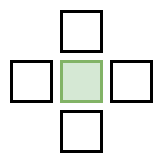
\includegraphics[width=0.4\textwidth]{figs/patterns/5point2DvonNeu.png}
		}
		\caption{5-point 2D von Neumann stencil}
		\label{fig:5p2DNeu}
	\end{subfigure}%
	\begin{subfigure}{.33\textwidth}
		\centering
		\fbox{
			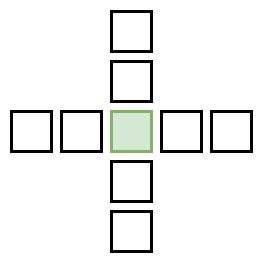
\includegraphics[width=0.6\textwidth]{figs/patterns/9point2DvonNeu.png}
		}
		\caption{9-point 2D von Neumann stencil}
		\label{fig:9p2DNeu}
	\end{subfigure}
	\begin{subfigure}{.33\textwidth}
		\centering
		\fbox{
			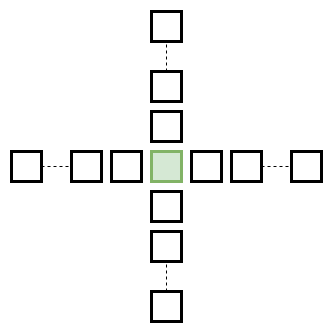
\includegraphics[width=0.6\textwidth]{figs/patterns/Npoint2DvonNeu.png}
		}
		\caption{N-point 2D von Neumann stencil}
		\label{fig:Np2DNeu}
	\end{subfigure}%
	\caption{Different 2D von Neuman stencils}
	\label{fig:2DvonNeu}
\end{figure}
The von Neumann stencils generalizes also to three dimensions.
The main idea is the same as for 2D but with an added dimension.
The number of read data points is thus more compared to the 2D case, and the number of \textit{N} points in a 3D von Neumann stencil can be formalized as $(N\bmod 6)=1\equiv true$.
Examples of 3D von Neumann stencil is seen in \autoref{fig:3DvonNeu}.
\begin{figure}[ht]
	\centering
	\begin{subfigure}{.33\textwidth}
		\centering
		\fbox{
			
\includegraphics[width=0.4\textwidth]{figs/patterns/7point3DNeu.png}
		}
		\caption{7-point 3D von Neumann stencil}
		\label{fig:7p3DNeu}
	\end{subfigure}%
	\begin{subfigure}{.33\textwidth}
		\centering
		\fbox{
			
\includegraphics[width=0.6\textwidth]{figs/patterns/13point3DNeu.png}
		}
		\caption{13-point 3D von Neumann stencil}
		\label{fig:13p3DNeu}
	\end{subfigure}
	\begin{subfigure}{.33\textwidth}
		\centering
		\fbox{
			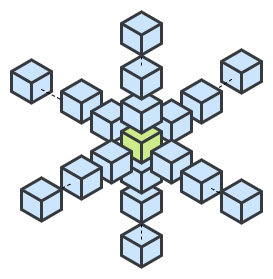
\includegraphics[width=0.6\textwidth]{figs/patterns/Npoint3DNeu.png}
		}
		\caption{N-point 3D von Neumann stencil}
		\label{fig:Np3DNeu}
	\end{subfigure}%
	\caption{Different 3D von Neuman stencils}
	\label{fig:3DvonNeu}
\end{figure}
\\\\
\textbf{Moore stencils} are almost the same as von Neumann stencils, with the exception that  they read \textit{all} neighbors relative to the input element.
This means that the shape of a 2D Moore stencil is a square, while the shape of a 3D Moore stencil is a cube.
The number of \textit{N} points in a 2D Moore stencil can be formalized as $(N\bmod 8)=1\equiv true$ and for the 3D case as $(N\bmod 26)=1\equiv true$.
Examples of Moore stencils is seen in \autoref{fig:Moore}.
\begin{figure}[ht]
	\centering
	\begin{subfigure}{.5\textwidth}
		\centering
		\fbox{
			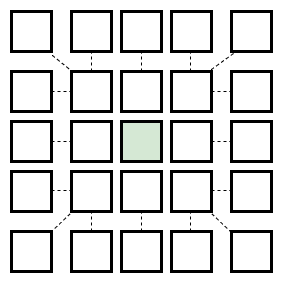
\includegraphics[width=0.4\textwidth]{figs/patterns/Np2dMoore.png}
		}
		\caption{N-point 2D Moore stencil}
		\label{fig:Np2DMoore}
	\end{subfigure}%
	\begin{subfigure}{.5\textwidth}
		\centering
		\fbox{
			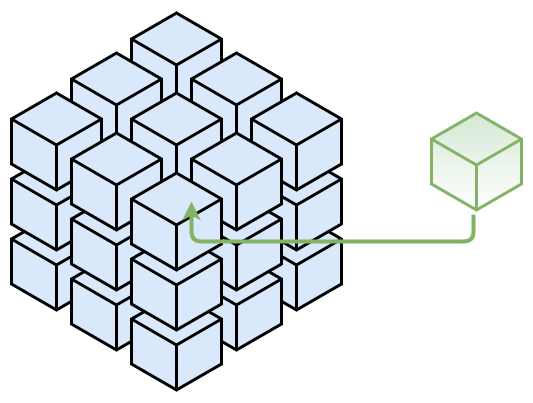
\includegraphics[width=0.6\textwidth]{figs/patterns/Np3dMoore.png}
		}
		\caption{27-point 3D Moore stencil}
		\label{fig:27p3DMoore}
	\end{subfigure}
	\caption{Different types of Moore stencils}
	\label{fig:Moore}
\end{figure}
As can be from \autoref{fig:27p3DMoore} the input element is surrounded by other other elements in the memory grid, and for this reason it is a bit difficult to illustrate that the input element resides inside the cube.
Notice that using 2D Moore stencils is a way of how kernels for image processing are implemented as described in \autoref{sec-gather}.
\\\\
An example of applying a 2D von Neumann stencil to an array of inputs is illustrated in \autoref{fig:2dMooreEx}.
In this case a thread is responsible for applying a single stencil to an input element.
\begin{figure}[ht]
	\centering
	\fbox{
		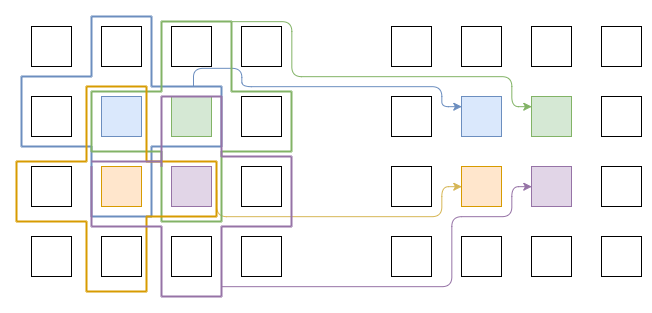
\includegraphics[width=0.6\textwidth]{figs/patterns/2dMooreEx.png}
	}
	\caption{Example of applying 2D Moore stencil}
	\label{fig:2dMooreEx}
\end{figure}
Implementing these stencils are done the same way as with the gather pattern, since stencils are special cases of this pattern.
In the case of applying stencils in parallel exploits a lot of data reuse since multiple threads are overlapping each other.
Implementing the stencil pattern maps very well to CUDA, since it is possible to represent both 2D and 3D structures in CUDA.
	
	\section{Transpose}
	\label{sec-transpose}
	The transpose communication pattern reorganizes a given data structure into its transpose representation.
Transpose is a special case of the scatter pattern since it writes its input into a different location in the output memory.

For example it might desirable to transpose a matrix which is represented by a 2D array, laid out in row-major order\footnote{Consecutive elements of a row reside next to each other}.
Transposing such a 2D array will lay out the matrix in column-major order in stead.
An example of transposing a 2D array using the scatter pattern is seen in \autoref{fig:transpose}.
Each thread reads an element from the array but writes its value somewhere scattered in memory according to its stride in the row column transpose.
In the example seen in \autoref{fig:transpose} the stride is three such that each input element with index $i$ will be scattered into "$i\bmod 3$" index in the output array.
\begin{figure}[ht]
	\centering
	\fbox{
		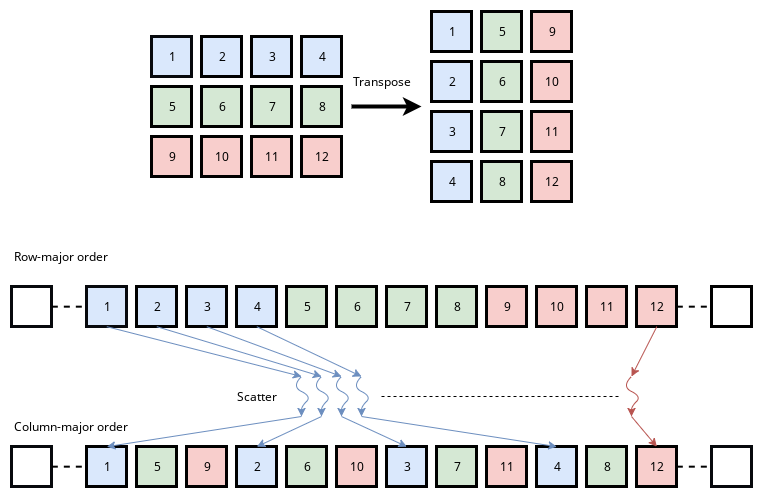
\includegraphics[width=0.6\textwidth]{figs/patterns/parallelTranspose.png}
	}
	\caption{Transpose Pattern}
	\label{fig:transpose}
\end{figure}
A major benefit for using the transpose pattern is that the input structure is reorganized into a more efficient memory structure since CUDA uses coalesced memory transactions when reading from and writing to memory.
The transpose pattern has many use case such as image processing, matrix algebra and more.
	

% citation test
\cite{McCool2012}
\cite{udacity:parallel}

\bibliographystyle{plain}
\bibliography{bib}

\end{document}
